\documentclass[11pt,a4paper]{article}
\usepackage[utf8]{inputenc}
\usepackage[T1]{fontenc}
\usepackage[brazil]{babel}
\usepackage{lmodern}
\usepackage[a4paper,margin=2.3cm]{geometry}
\usepackage{graphicx,booktabs,amsmath,xcolor,caption,float,enumitem}
\usepackage[hidelinks]{hyperref}
\definecolor{verde}{HTML}{1F5C3A}
\captionsetup{font=small,labelfont=bf}
\setlist{itemsep=2pt,topsep=4pt}
\usepackage{titlesec}
\titleformat{\section}{\large\bfseries\color{verde}}{\thesection}{0.6em}{}
\titleformat{\subsection}{\normalsize\bfseries\color{verde}}{\thesubsection}{0.6em}{}
\begin{document}

\begin{center}
{\small PROGRAMA CENTELHA 3 PARANÁ \textbar{} RELATÓRIO TÉCNICO RT-01}\\[6pt]
{\LARGE\bfseries\color{verde} SPECULA}\\[4pt]
{\large Prova de conceito por simulação:\\ detectabilidade óptica e suficiência do desenho de coleta}\\[8pt]
Anuar José Mincache\\
Maringá, novembro de 2026 \textbar{} versão 0.1 (beta)\\[2pt]{\small Código, dados e figuras: \url{https://github.com/anuarmincache/specula-rt01}}
\end{center}

\begin{center}
\fbox{\parbox{0.9\textwidth}{\small\textbf{Natureza deste documento.} Este relatório apresenta \emph{simulações}, não experimentos. Nenhum instrumento foi montado e nenhuma folha foi medida. O estágio da solução continua sendo \textbf{Ideia}. As simulações usam um modelo físico publicado e validado (PROSPECT-D), a especificação de fábrica do sensor e dados epidemiológicos publicados da ferrugem do cafeeiro. Elas servem para testar, antes de gastar recurso, se o sensor escolhido tem chance de enxergar o fenômeno e se a coleta de campo planejada produz dados suficientes. Todas as hipóteses estão declaradas e todo o código é reproduzível.}}
\end{center}

\section*{Resumo}
\textbf{Simulação 1.} Folhas de café foram simuladas com o modelo PROSPECT-D e medidas por um modelo do sensor AS7265x (18 bandas de 20 nm). Quando a folha infectada é comparada com \emph{outras} folhas sadias, a variação natural entre folhas esconde o sinal: com alteração de 10\% nos pigmentos e na matéria seca, a área sob a curva ROC (AUC) fica em 0,62. Quando a folha é comparada com \emph{ela mesma} em visitas anteriores (autorreferência), a mesma alteração atinge AUC de 0,99, e uma alteração de 5\% já atinge 0,90. Com autorreferência, as 18 bandas do AS7265x têm desempenho equivalente a um espectrômetro de referência e superior a uma câmera de três bandas largas.

\textbf{Simulação 2.} Um modelo Monte Carlo da coorte de 1.500 folhas etiquetadas em Cambira (PR), com incubação calculada pelo clima local e progresso da doença ancorado em dados de campo publicados, mostra que a coorte gera cerca de 232 folhas positivas com incidência de 20\% e mais de 96 positivas (o necessário para estimar a sensibilidade com margem de $\pm$10 pontos) sempre que a incidência final passa de 10\% e a perda de folhas fica em até 1\% por semana. A simulação também mostrou uma falha no calendário original: como as lesões aparecem sobretudo entre março e maio, concentrar as visitas em dezembro a fevereiro dá apenas 4 medições antes do sintoma por folha (mediana). Um calendário ajustado à epidemia, com 4 visitas a mais, dobra esse número para 8.

\section{Objetivo e perguntas}
O SPECULA propõe medir a refletância de folhas de café no visível e no infravermelho próximo para antecipar a ferrugem (\emph{Hemileia vastatrix}). Antes de comprar hardware, duas perguntas precisam de resposta quantitativa:
\begin{enumerate}
\item \textbf{O sensor enxerga?} Um sensor de baixo custo com 18 bandas de 20 nm consegue distinguir as alterações que a literatura descreve nas primeiras semanas da infecção, considerando o ruído de medição e a variação natural entre folhas?
\item \textbf{A coleta gera dados suficientes?} A coorte de 1.500 folhas etiquetadas, com o calendário de visitas do cronograma, produz folhas doentes e medições anteriores ao sintoma em quantidade suficiente para treinar e validar um modelo?
\end{enumerate}

\section{Simulação 1: detectabilidade óptica}
\subsection{Modelo da folha}
A refletância foi calculada com o PROSPECT-D \cite{feret2017}, a versão atual do modelo de placas de Jacquemoud e Baret \cite{jacquemoud1990}, implementada no pacote \texttt{prosail} \cite{prosail}. O modelo calcula a refletância de 400 a 2500 nm a partir de seis parâmetros: estrutura do mesofilo ($N$), clorofila ($C_{ab}$), carotenoides ($C_{ar}$), pigmentos marrons, espessura equivalente de água ($C_w$) e matéria seca por área ($C_m$). A Tabela~\ref{tab:param} lista os valores e a origem de cada um.

\begin{table}[H]\centering\footnotesize\setlength{\tabcolsep}{4pt}
\caption{Parâmetros da folha sadia de referência, variação natural e origem.}\label{tab:param}
\begin{tabular}{lcccl}\toprule
Parâmetro & Valor & CV entre folhas & CV no tempo & Origem \\\midrule
$N$ (estrutura) & 1,5 & 5\% & 0,5\% & Soares et al. \cite{soares2022}, que usaram $N=1{,}5$ para café \\
$C_{ab}$ ($\mu$g cm$^{-2}$) & 45 & 15\% & 2\% & valor típico de folha verde madura (hipótese) \\
$C_{ar}$ ($\mu$g cm$^{-2}$) & 10 & 15\% & 2\% & razão típica $C_{ar}/C_{ab}$ (hipótese) \\
$C_w$ (g cm$^{-2}$) & 0,015 & 10\% & 2\% & folha coriácea (hipótese) \\
$C_m$ (g cm$^{-2}$) & 0,009 & 10\% & 1\% & 90 g m$^{-2}$ de massa por área (hipótese) \\
Pigmentos marrons & 0 & & & folhas verdes, como em \cite{soares2022} \\\bottomrule
\end{tabular}
\end{table}
\noindent Os valores marcados como hipótese serão substituídos por medições na fase de bancada do projeto. Os resultados dependem mais das \emph{variações} relativas do que dos valores absolutos, e a análise foi repetida para dois níveis de ruído.

\subsection{Cenários de alteração precoce}
Soares et al. \cite{soares2022} inocularam 160 mudas de `Mundo Novo' com \emph{H.~vastatrix} e compararam com 160 controles. Aos 15 dias após a inoculação, ainda sem sintomas, encontraram diferenças significativas em carotenoides e matéria seca (maiores nas inoculadas) e em espessura de água (menor), sem diferença na clorofila. Com imagens de três bandas e SVM, separaram os grupos com 80\% de acerto (kappa 0,6). O artigo não publica a magnitude das alterações, então a simulação varia o \emph{tamanho do efeito} $s$ de 0 a 20\%:
\begin{itemize}
\item \textbf{Cenário A} (direções de Soares et al. aos 15 dias): $C_{ar}\times(1+s)$, $C_m\times(1+s)$, $C_w\times(1-s)$, clorofila inalterada.
\item \textbf{Cenário B} (fase posterior): perda de clorofila, $C_{ab}\times(1-s)$. A queda de eficiência fotoquímica antes do sintoma visual também foi descrita por imagem de fluorescência \cite{honorato2015}.
\end{itemize}

\subsection{Modelo do sensor}
O AS7265x tem 18 canais centrados em 410, 435, 460, 485, 510, 535, 560, 585, 610, 645, 680, 705, 730, 760, 810, 860, 900 e 940 nm, com largura a meia altura de 20 nm e conversor de 16 bits \cite{as7265x}. Cada canal foi modelado como um filtro gaussiano aplicado ao espectro do PROSPECT-D. O ruído de medição foi modelado como multiplicativo, com desvio relativo de 1\% e de 2\% por canal. Para sensores da mesma família, Besozzi et al. \cite{besozzi2026} mediram coeficientes de variação de $10^{-4}$ a $10^{-2}$ em condição controlada; os valores adotados são mais conservadores para incluir o reposicionamento da ponteira na folha.

\subsection{Desenho estatístico}
Para cada tamanho de efeito foram simuladas 200 folhas sadias e 200 alteradas, cada uma com parâmetros sorteados segundo a variação natural da Tabela~\ref{tab:param}. Dois modos foram comparados:
\begin{itemize}
\item \textbf{Comparação entre folhas:} a medição de uma folha alterada é comparada com a de outras folhas sadias.
\item \textbf{Autorreferência:} cada folha tem uma linha de base (média de 4 visitas anteriores, com deriva natural no tempo e ruído), e o classificador recebe a diferença entre a medição atual e a linha de base da \emph{mesma} folha. É exatamente o que a coorte de folhas etiquetadas permite.
\end{itemize}
O classificador foi a análise discriminante linear sobre o logaritmo da refletância, avaliada por validação cruzada estratificada de 5 partes, com 3 repetições independentes \cite{sklearn}. A métrica é a AUC: 0,5 equivale ao acaso e 1,0 à separação perfeita.

\subsection{Resultados}
\begin{figure}[H]\centering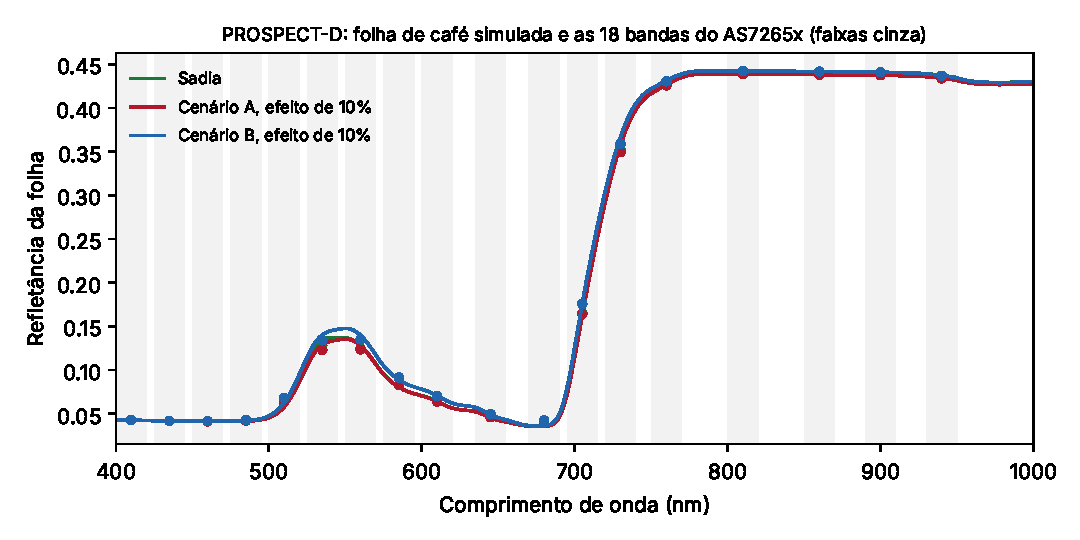
\includegraphics[width=0.92\textwidth]{fig/fig1_espectros.pdf}
\caption{Refletância simulada da folha sadia e alterada (10\%) e as bandas do AS7265x. As diferenças são pequenas a olho nu, o que justifica a análise estatística a seguir.}\end{figure}

\begin{figure}[H]\centering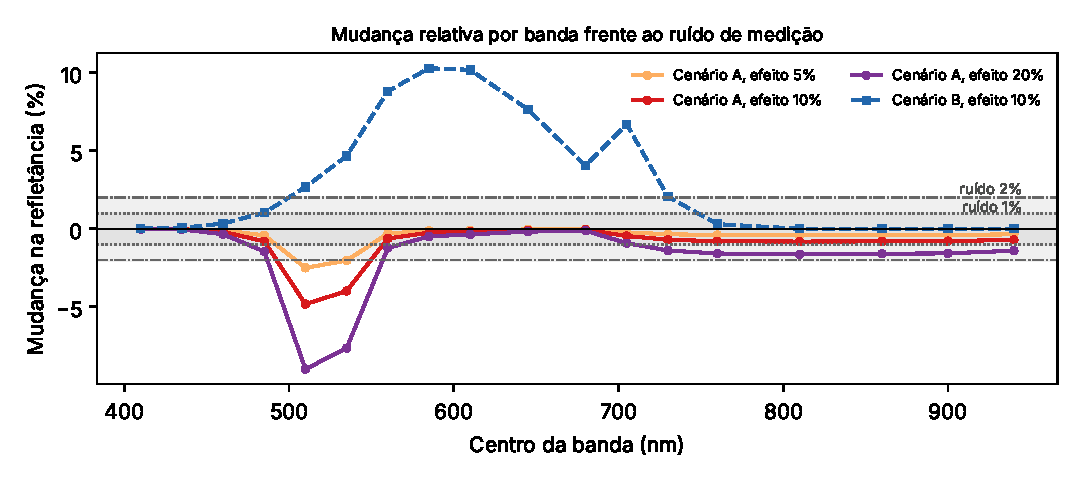
\includegraphics[width=0.92\textwidth]{fig/fig2_bandas.pdf}
\caption{Mudança relativa em cada banda. No cenário A, a assinatura se concentra em 510 e 535 nm (região de absorção dos carotenoides): -4,8\% e -4,0\% com efeito de 10\%. No cenário B, a assinatura está entre 560 e 705 nm, chegando a +10,3\% em 585 nm. As faixas cinza indicam o ruído de 1\% e de 2\%.}\end{figure}

\begin{figure}[H]\centering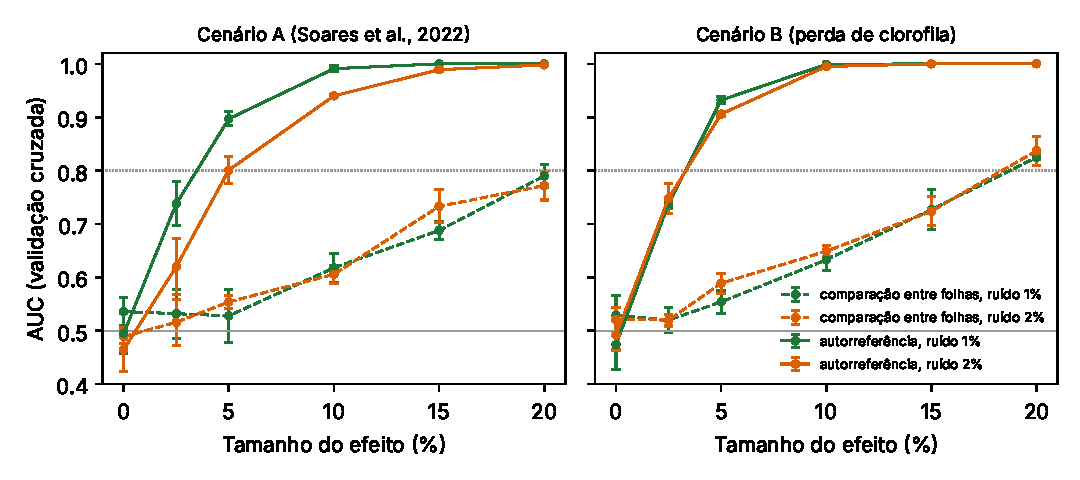
\includegraphics[width=0.95\textwidth]{fig/fig3_auc.pdf}
\caption{Detectabilidade em função do tamanho do efeito. Linhas tracejadas: comparação entre folhas. Linhas cheias: autorreferência. Barras: desvio padrão entre 3 repetições.}\label{fig:auc}\end{figure}

\begin{table}[H]\centering\small
\caption{AUC por modo de análise e tamanho do efeito (ruído de 1\%).}\label{tab:auc}
\begin{tabular}{lcccc}\toprule
 & \multicolumn{2}{c}{Cenário A} & \multicolumn{2}{c}{Cenário B} \\\cmidrule(lr){2-3}\cmidrule(lr){4-5}
Efeito & entre folhas & autorreferência & entre folhas & autorreferência \\\midrule
2,5\% & 0,53 & 0,74 & 0,52 & 0,74 \\
5\% & 0,53 & 0,90 & 0,55 & 0,93 \\
10\% & 0,62 & 0,99 & 0,63 & 1,00 \\
20\% & 0,79 & 1,00 & 0,82 & 1,00 \\\bottomrule
\end{tabular}
\end{table}

\begin{figure}[H]\centering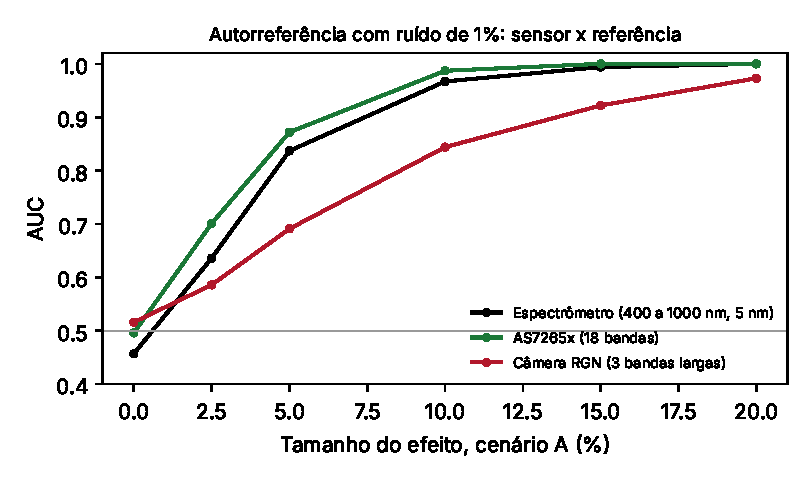
\includegraphics[width=0.66\textwidth]{fig/fig4_sensores.pdf}
\caption{Autorreferência com ruído de 1\%, cenário A, para três configurações de sensor: espectrômetro de 400 a 1000 nm com passo de 5 nm, AS7265x e câmera de três bandas largas (550, 660 e 850 nm, como a usada por Soares et al.).}\label{fig:sens}\end{figure}

\subsection{O que a simulação 1 mostra}
\begin{enumerate}
\item \textbf{A variação natural entre folhas é o obstáculo principal, não o ruído do sensor.} Comparando folhas diferentes, um efeito de 10\% dá AUC de apenas 0,62. Isso explica por que diagnósticos de imagem única tendem a funcionar só depois do sintoma.
\item \textbf{A autorreferência resolve o problema.} Medindo a mesma folha ao longo do tempo, o efeito de 5\% chega a AUC 0,90 (cenário A) e 0,93 (cenário B), e o de 10\% passa de 0,94 mesmo com ruído de 2\%. É a justificativa quantitativa da coorte de folhas etiquetadas e do nó Sentinel, que mede a mesma folha todos os dias.
\item \textbf{O AS7265x é suficiente.} Com efeito de 5\%, o AS7265x atinge 0,87, contra 0,84 do espectrômetro e 0,69 da câmera de três bandas. O espectrômetro não leva vantagem aqui porque muitas variáveis com poucas amostras penalizam o classificador linear; com mais dados ele pode superar o sensor. A câmera de três bandas perde a região de 510 a 535 nm, onde está a assinatura do cenário A. Os três sensores usam o mesmo classificador linear, então a diferença vem só das bandas, não do algoritmo. Os 80\% de Soares et al. vêm de outro classificador (SVM) e de outro desenho experimental e não são diretamente comparáveis a estes valores.
\end{enumerate}

\section{Simulação 2: suficiência da coorte de campo}
\subsection{Desenho simulado}
A simulação reproduz o cronograma original do projeto: 1.500 folhas do 3º e 4º par de ramos do terço médio, etiquetadas em 01/12/2027, com 2 visitas por semana até 29/02/2028 e 1 visita por semana até 15/05/2028. São 34 visitas mais a medição da etiquetagem, ou 35 medições por folha. Por ter menos visitas na fase de maior progresso da doença, esse calendário é o caso conservador e é o usado nos cenários abaixo. Cada realização sorteia, para cada folha, se ela adoece, quando a lesão aparece, quando ocorreu a infecção e se a folha é perdida. Foram feitas 300 realizações por cenário.

\subsection{Período de incubação pelo clima local}
O período de incubação (da infecção ao sintoma) foi calculado mês a mês por duas equações revisadas por Alfonsi et al. \cite{alfonsi2019}: Ortolani et al. (1971), $Y = 63{,}47 - 1{,}526\,\bar{T}$, e Moraes et al. (1976), $Y = 93{,}27 - 0{,}99\,T_{\max} - 1{,}51\,T_{\min}$, com as temperaturas médias mensais de Apucarana, município vizinho à área experimental \cite{climatempo}. Foi aplicada variação aleatória de $\pm$15\% em torno do valor do mês. A Tabela~\ref{tab:ip} mostra que os valores ficam dentro da faixa de 28 a 65 dias relatada para o Brasil \cite{alfonsi2019}; para Maringá e Londrina, a literatura citada por esses autores indica 30 e 31 dias.

\begin{table}[H]\centering\small
\caption{Período de incubação estimado para Cambira (dias).}\label{tab:ip}
\begin{tabular}{lcc}\toprule
Mês & Ortolani et al. & Moraes et al. \\\midrule
Dezembro & 27,6 & 36,9 \\
Janeiro & 26,8 & 35,3 \\
Fevereiro & 26,8 & 35,3 \\
Março & 28,4 & 37,8 \\
Abril & 30,7 & 41,9 \\
Maio & 35,2 & 49,4 \\
Junho & 36,8 & 51,9 \\\bottomrule
\end{tabular}
\end{table}

\subsection{Progresso da doença e perdas}
Em lavouras sem controle químico, a ferrugem começa em dezembro e atinge o pico entre maio e julho, segundo 6 anos de monitoramento mensal em Varginha (MG) com 100 folhas do 3º e 4º par do terço médio \cite{japiassu2005,meira2009}. No sul de Minas, o pico chegou a 87,5\% e 91\% sem controle químico e ficou em 15\% com controle convencional \cite{lopes2012}. A fração de folhas etiquetadas que mostram lesão foi modelada por uma curva logística com início em dezembro e ponto médio em 1º de abril, e a incidência final foi variada entre 10\% e 70\% para cobrir desde lavoura com controle até lavoura sem controle (faixa com manejo reduzido prevista no projeto). A perda de folhas ou etiquetas (queda natural, poda, dano) foi modelada como taxa semanal constante de 0,5\%, 1\% e 2\%.

\subsection{Critério de suficiência}
O resultado técnico do projeto é a sensibilidade do sistema a uma dada antecedência. Para estimar uma proporção com intervalo de confiança de 95\% de $\pm$10 pontos no pior caso ($p=0{,}5$) são necessárias $n = 1{,}96^2 \times 0{,}25 / 0{,}10^2 \approx 96$ folhas positivas com medição naquela antecedência. Adotamos como critério ter pelo menos 96 folhas positivas com medição entre 14 e 21 dias antes da lesão.

\subsection{Resultados}
\begin{figure}[H]\centering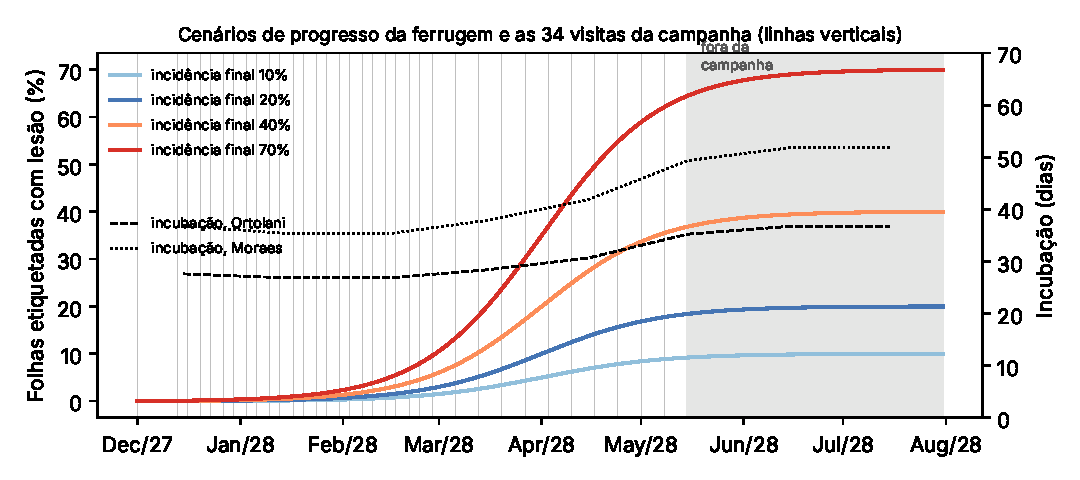
\includegraphics[width=0.95\textwidth]{fig/fig5_progresso.pdf}
\caption{Cenários de progresso da doença nas folhas etiquetadas, datas das visitas e período de incubação mês a mês pelas duas equações.}\end{figure}

\begin{table}[H]\centering\footnotesize\setlength{\tabcolsep}{4pt}
\caption{Resultados por incidência final (perda de 1\% por semana, salvo indicação). Positivas: mediana e intervalo de 5\% a 95\% das 300 realizações.}\label{tab:coorte}
\begin{tabular}{lccccc}\toprule
Incidência & Positivas detectadas & \multicolumn{2}{c}{Medições pré-sintoma (mediana)} & \multicolumn{2}{c}{Prob. de $\geq$96 positivas a 14 a 21 dias} \\\cmidrule(lr){3-4}\cmidrule(lr){5-6}
final & (Ortolani) & Ortolani & Moraes & perda 1\%/sem. & perda 2\%/sem. \\\midrule
10\% & 116 [100; 133] & 4 & 6 & 100\% & 66\% \\
20\% & 232 [211; 254] & 4 & 6 & 100\% & 100\% \\
40\% & 466 [438; 495] & 4 & 6 & 100\% & 100\% \\
70\% & 816 [785; 845] & 4 & 6 & 100\% & 100\% \\
\bottomrule
\end{tabular}
\end{table}

\begin{figure}[H]\centering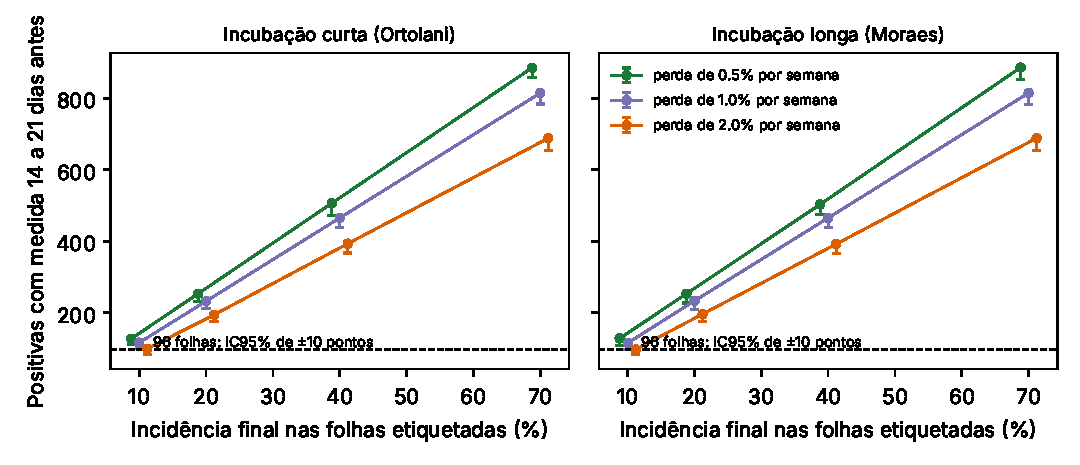
\includegraphics[width=0.95\textwidth]{fig/fig6_positivos.pdf}
\caption{Folhas positivas com medição entre 14 e 21 dias antes da lesão. Pontos: mediana. Barras: percentil 5. Linha tracejada: 96 folhas.}\end{figure}

\begin{figure}[H]\centering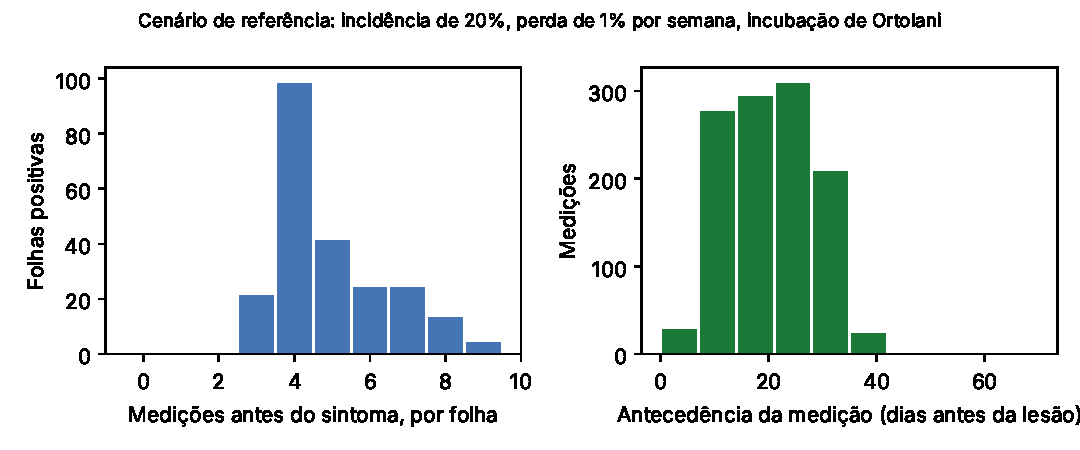
\includegraphics[width=0.95\textwidth]{fig/fig7_antecedencia.pdf}
\caption{Cenário de referência (incidência de 20\%): medições antes do sintoma por folha e distribuição da antecedência de todas as medições pré-sintomáticas.}\end{figure}

\begin{figure}[H]\centering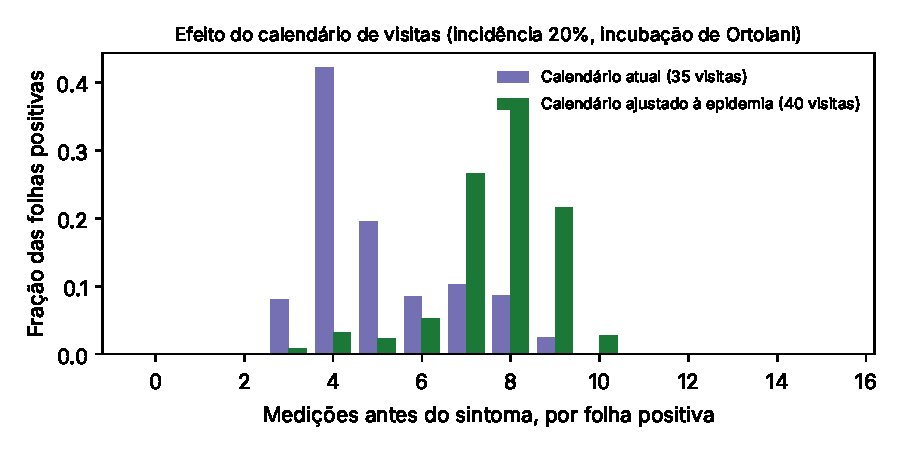
\includegraphics[width=0.72\textwidth]{fig/fig8_calendarios.pdf}
\caption{Calendário original (visitas intensivas de dezembro a fevereiro) contra calendário ajustado à epidemia, adotado no cronograma final (semanal do fim da etiquetagem a janeiro, duas por semana de 01/02 a 15/05/2028). As contagens excluem a medição da etiquetagem.}\label{fig:cal}\end{figure}

\subsection{O que a simulação 2 mostra}
\begin{enumerate}
\item \textbf{A coorte de 1.500 folhas é suficiente se a incidência final passar de 10\%.} Com 20\%, a coorte gera 232 positivas (mediana). Com 10\% e perda de 1\% por semana, gera 116 e cumpre o critério em 100\% das realizações; com perda de 2\% por semana, a chance cai para 66\%. Por isso o projeto prevê uma faixa com manejo reduzido de fungicida e etiquetagem com sobra.
\item \textbf{O calendário original estava mal alinhado com a epidemia.} A maioria das lesões aparece entre março e maio, quando o calendário original tem só uma visita por semana. O resultado é uma mediana de 4 medições antes do sintoma por folha (6 com a incubação mais longa). Com o calendário ajustado, de 38 visitas mais a etiquetagem, a mediana sobe para 8 (10), e a fração de folhas com pelo menos 6 medições pré-sintomáticas passa de 30\% para 93\%. O custo é de 4 visitas a mais.
\item \textbf{O Marco 3 precisa ser reposicionado.} Com incidência final de 20\%, espera-se cerca de 43 folhas com lesão até 29/02/2028 e 146 até 31/03/2028. O critério original (60 folhas até o fim de fevereiro) falharia mesmo num cenário bom. O critério coerente com a simulação é manter as 60 folhas, mas verificá-las em 31/03/2028: com incidência final de 10\% e perda de 1\% por semana, esperam-se cerca de 60 a 65 folhas com lesão nessa data, e 10\% é justamente o mínimo que dá poder estatístico.
\end{enumerate}

\section{Decisões de projeto que saem das simulações}
\begin{itemize}
\item Manter a medição repetida da mesma folha (coorte e Sentinel) como base do método, porque é ela que torna a alteração precoce detectável.
\item Manter o AS7265x como sensor do Scan; não usar câmeras de três bandas como fonte espectral.
\item Ajustar o calendário de campo: semanal do fim da etiquetagem até 31/01/2028 e duas visitas por semana de 01/02 a 15/05/2028 (38 visitas mais a etiquetagem, cerca de 58,5 mil medições). Já adotado no cronograma do projeto.
\item Reposicionar o Marco 3 para 31/03/2028, mantendo o critério de pelo menos 60 folhas com lesão. Já adotado no cronograma do projeto.
\item Garantir incidência mínima de 10\% com faixa de manejo reduzido e manter a perda de folhas em até 1\% por semana, com etiquetagem de sobra.
\end{itemize}

\section{Limitações}
\begin{itemize}
\item As magnitudes das alterações foliares aos 15 dias não foram publicadas por Soares et al.; por isso os efeitos foram varridos de 0 a 20\%. O tamanho real do efeito em folha adulta no campo só será conhecido com a coleta.
\item No cenário A o PROSPECT-D prevê leve queda no infravermelho próximo, enquanto Soares et al. relatam aumento medido por drone. A diferença pode vir de mudanças de estrutura do mesofilo ($N$), não medidas no artigo, ou de efeitos de dossel. A detecção simulada não depende do infravermelho próximo, e sim da região de 510 a 535 nm.
\item Os valores de clorofila, carotenoides, água e matéria seca da folha sadia e suas variações são hipóteses, a substituir por medições na bancada.
\item A curva de progresso da doença foi ancorada no calendário e nos picos publicados, não ajustada a dados de Cambira. O histórico da propriedade será levantado antes da campanha.
\item A simulação não inclui outras doenças nem estresses que imitam a ferrugem; esse risco é tratado no projeto pela avaliação agronômica e pela confirmação do patógeno em laboratório.
\end{itemize}

\section{Reprodutibilidade}
\sloppy As duas simulações estão em Python (\texttt{sim\_optica.py} e \texttt{sim\_coorte.py}), com sementes fixas (20261111 e 20261112), e usam \texttt{prosail}, \texttt{numpy}, \texttt{scikit-learn} e \texttt{matplotlib}, com as versões travadas em \texttt{requirements.txt}. Os resultados numéricos completos estão em \texttt{resultados\_optica.json} e \texttt{resultados\_coorte.json}, e todos os números deste relatório são lidos desses arquivos. Repositório público: \url{https://github.com/anuarmincache/specula-rt01}.

\begin{thebibliography}{99}\small
\bibitem{alfonsi2019} ALFONSI, W. M. V.; COLTRI, P. P.; ZULLO JÚNIOR, J.; PATRÍCIO, F. R. A.; ALFONSI, E. L. Período de incubação da ferrugem do cafeeiro. \textit{Summa Phytopathologica}, v. 45, n. 2, p. 134-140, 2019. doi:10.1590/0100-5405/187216.
\bibitem{as7265x} AMS OSRAM. \textit{AS7265x Smart 18-Channel VIS to NIR Spectral\_ID 3-Sensor Chipset with Electronic Shutter}. Datasheet. Disponível em: cdn.sparkfun.com/assets/c/2/9/0/a/AS7265x\_Datasheet.pdf.
\bibitem{besozzi2026} BESOZZI, A.; GIBERTONI, G.; ROVATI, L.; GIBALDI, A. Flexible calibration method: photometric and radiometric measurements with compact low-cost multi-channel sensors. \textit{Acta IMEKO}, v. 15, n. 2, p. 1-12, 2026. doi:10.21014/actaimeko.v15i2.2267.
\bibitem{climatempo} CLIMATEMPO. Climatologia de Apucarana (PR), médias de 30 anos. Disponível em: climatempo.com.br/climatologia/1301/apucarana-pr. Acesso em: 11 nov. 2026.
\bibitem{feret2017} FÉRET, J.-B.; GITELSON, A. A.; NOBLE, S. D.; JACQUEMOUD, S. PROSPECT-D: towards modeling leaf optical properties through a complete lifecycle. \textit{Remote Sensing of Environment}, v. 193, p. 204-215, 2017. doi:10.1016/j.rse.2017.03.004.
\bibitem{prosail} GÓMEZ-DANS, J. L. \textit{prosail}: Python bindings for the PROSPECT and SAIL models. Pacote Python. Disponível em: github.com/jgomezdans/prosail.
\bibitem{honorato2015} HONORATO JÚNIOR, J.; ZAMBOLIM, L.; DUARTE, H. S. S.; AUCIQUE-PÉREZ, C. E.; RODRIGUES, F. A. Effects of epoxiconozale and pyraclostrobin fungicides in the infection process of \textit{Hemileia vastatrix} on coffee leaves as determined by chlorophyll \textit{a} fluorescence imaging. \textit{Journal of Phytopathology}, v. 163, n. 11-12, p. 968-977, 2015. doi:10.1111/jph.12399.
\bibitem{jacquemoud1990} JACQUEMOUD, S.; BARET, F. PROSPECT: a model of leaf optical properties spectra. \textit{Remote Sensing of Environment}, v. 34, n. 2, p. 75-91, 1990. doi:10.1016/0034-4257(90)90100-Z.
\bibitem{japiassu2005} JAPIASSÚ, L. B.; GARCIA, A. W. R.; MIGUEL, A. E.; MENDONÇA, J. M. A.; CARVALHO, C. H. S.; FERREIRA, R. A.; MATIELLO, J. B. Influência da carga pendente, do espaçamento e de fatores climáticos no desenvolvimento da ferrugem do cafeeiro. In: SIMPÓSIO DE PESQUISA DOS CAFÉS DO BRASIL, 4., 2005, Londrina. \textit{Anais}. Brasília: Embrapa Café, 2005.
\bibitem{lopes2012} LOPES, P. R.; FERRAZ, J. M. G.; THEODORO, V. C. A.; LOPES, I. M. Evolução da ferrugem e da cercosporiose em agroecossistemas cafeeiros convencional, organo-mineral e orgânico. \textit{Revista Brasileira de Agroecologia}, v. 7, n. 1, p. 160-168, 2012.
\bibitem{meira2009} MEIRA, C. A. A.; RODRIGUES, L. H. A. Árvore de decisão na análise de epidemias da ferrugem do cafeeiro. In: SIMPÓSIO DE PESQUISA DOS CAFÉS DO BRASIL, 6., 2009, Vitória. \textit{Anais}. Vitória: Consórcio Pesquisa Café, 2009.
\bibitem{sklearn} PEDREGOSA, F. et al. Scikit-learn: machine learning in Python. \textit{Journal of Machine Learning Research}, v. 12, p. 2825-2830, 2011.
\bibitem{soares2022} SOARES, A. S.; VIEIRA, B. S.; BEZERRA, T. A.; MARTINS, G. D.; SIQUIEROLI, A. C. S. Early detection of coffee leaf rust caused by \textit{Hemileia vastatrix} using multispectral images. \textit{Agronomy}, v. 12, n. 12, 2911, 2022. doi:10.3390/agronomy12122911.
\end{thebibliography}

\vspace{1em}
\begin{center}
\fcolorbox{verde}{white}{\parbox{0.9\textwidth}{\centering\small
\textbf{\color{verde}Acesso aberto para a banca avaliadora}\\[4pt]
Todo o código, os dados de entrada, os resultados numéricos e as figuras deste relatório estão disponíveis em\\[4pt]
{\large\url{https://github.com/anuarmincache/specula-rt01}}\\[4pt]
Versão 0.1 (beta). Qualquer número do relatório pode ser reproduzido com os scripts do repositório.}}
\end{center}
\end{document}
